
\section{Aufbau der Messeinrichtung}

\begin{figure}[H]
\centering
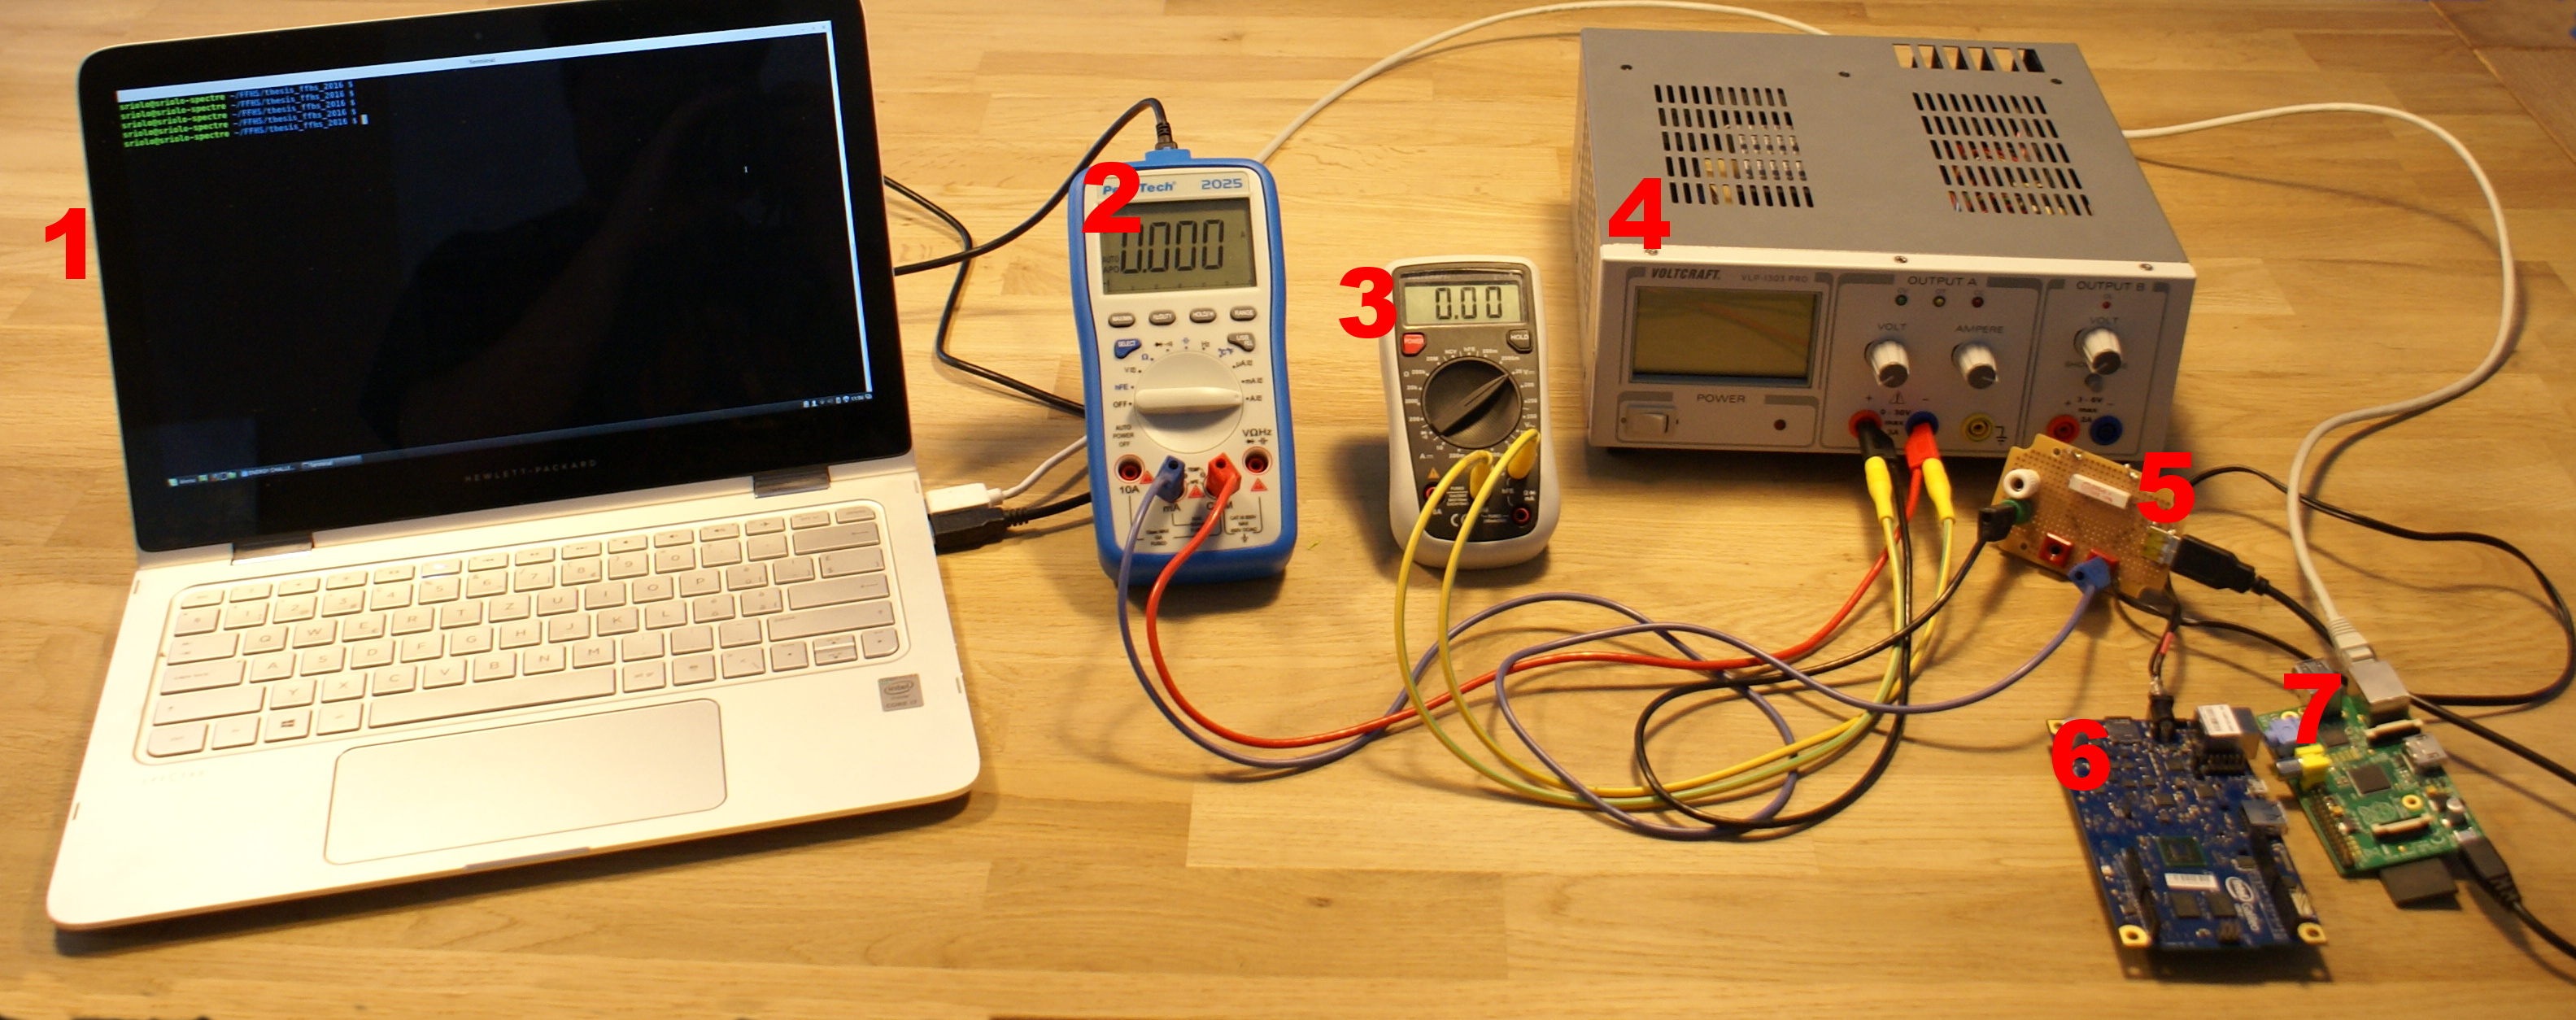
\includegraphics[width=1.0\textwidth]{images/setup.jpg}
\caption{Aufbau der Messeinrichtung}
\label{fig:Setup}
\end{figure}

\autoref{fig:Setup} enthält eine Übersicht der für die Messung notwendigen Bestandteile. Diese sind: 1.) Ein PC, der die Benchmarks auf dem SoC ausführt und die gemessenen Daten entgegennimmt. 2.) Das Messgerät, das den Strom misst und die Daten über eine USB-Schnittstelle an den PC weiterleitet. 3.) Ein optionales Messgerät, damit die Spannung des Spannungsreglers überprüft werden kann. 4.) Ein Spannungsregler, der eine konstante Spannung sicherstellt. 5.) Ein Verteiler, damit ein Galileo oder Raspberry Pi Board angeschlossen werden kann. Ansonsten hat der Verteiler keine elektronischen Eigenschaften. 6.) Das Galileo Board. 7.) Das Raspberry Pi Board.

